\section{Proyectos}

\begin{frame}{Pequeños Proyectos}[Carro para telemetría]
	
	% \begin{figure}[H]
	% 	\centering
	% 	\includegraphics[width=0.5\textwidth]{imgs/carro}
	% 	\caption[]{}
	% \end{figure}

\end{frame} 
     
\begin{frame}{Caracteristicas}
	\begin{itemize}
		\item protocolos de comunicación: Bluetooth, Wifi, RadioFrecuencia.
		\item	actuadores:  motores o brazos mecánicos.
		\item 	Sensores: Luz, Sonido, Temperatura, Humedad, Distancia (Ultrasonido), Posición (Giroscopio), ubicación (GPS).
		\item 	Cámara: reconocimiento de Objetos, Realidad Aumentada. 
	\end{itemize}
\end{frame}

\begin{frame}{Condiciones Laborales}
	\begin{itemize}
	 		\item senseo de Sonido y Temperatura para el 4to piso del bl 19
	 		\item almacenamiento, procesamiento y presentación de datos.
	 	\end{itemize} 	

\end{frame}


\begin{frame}{Multirotores}
	
	\begin{figure}[H]
		\centering
		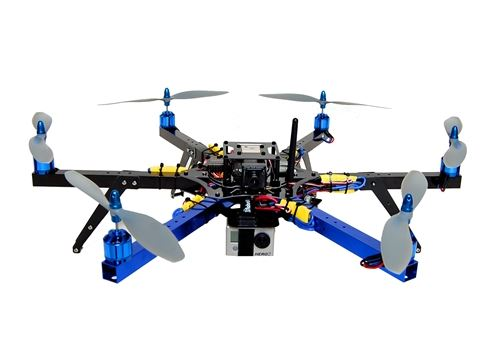
\includegraphics[width=0.5\textwidth]{imgs/ardu-hexaARF-gopro}
		\caption{Hexacopter}
	\end{figure}
	
\end{frame}
